
%*******************************************************************************
%*********************************** Second Chapter ***************************
%*******************************************************************************
%!TEX root = 0.main.tex

\section{Non uniform sampling schemes and other Discrete Laplacians}

In a Graph Spherical CNN we use the fact that when the sampling scheme of the sphere is regular enough, the graph $W_{i j} = \exp {-\frac{\norm{x_i-x_j}^2}{4t}}$ is such that the corresponding graph Laplacian $\mathbf L_n^t$ has a spectrum that is close enough to the spectrum of $\triangle_{\mathbb S^2}$. In this way we can approximate a spherical convolution of a signal $f$ with a kernel $h$ with the graph convolution of the sampled signal $\mathbf f$
$$
V\text{diag}\{h(\lambda_0), ..., h(\lambda_{n-1})\}V^T\mathbf f
$$
In Chapter 2 we showed a way to construct $\mathbf L_n^t$ that well approximates $\triangle_{\mathbb S^2}$ in the case of a regular sampling scheme of the sphere. In this Chapter we focus on other sampling schemes less uniform than HEALPix. The sampling scheme that we will use for our study, very used in applications, is the so called \textit{equiangular sampling scheme}. We observe that in this case the HKGL is not able to correctly approximate the continuous Laplace-Beltrami operator, due to the fact that the equiangular sampling samples the areas near the poles more than the area close to the equator. Figure \ref{fig:equiangular distortion} well illustrates this bad behavior of the HKGL. To better show the distortion caused by the HKGL, in figure \ref{fig:equiangular distortion} the sphere was sampled with many more samples near the poles than near the equator. The sample points are shown as the vertices of the triangulation used for the plot. On the left we plot one spherical harmonic $Y_\ell^m$ of degree $\ell=4$ and on the right we plot the corresponding eigenmode of the HKGL. 
\begin{figure}[h]
	\begin{center}
		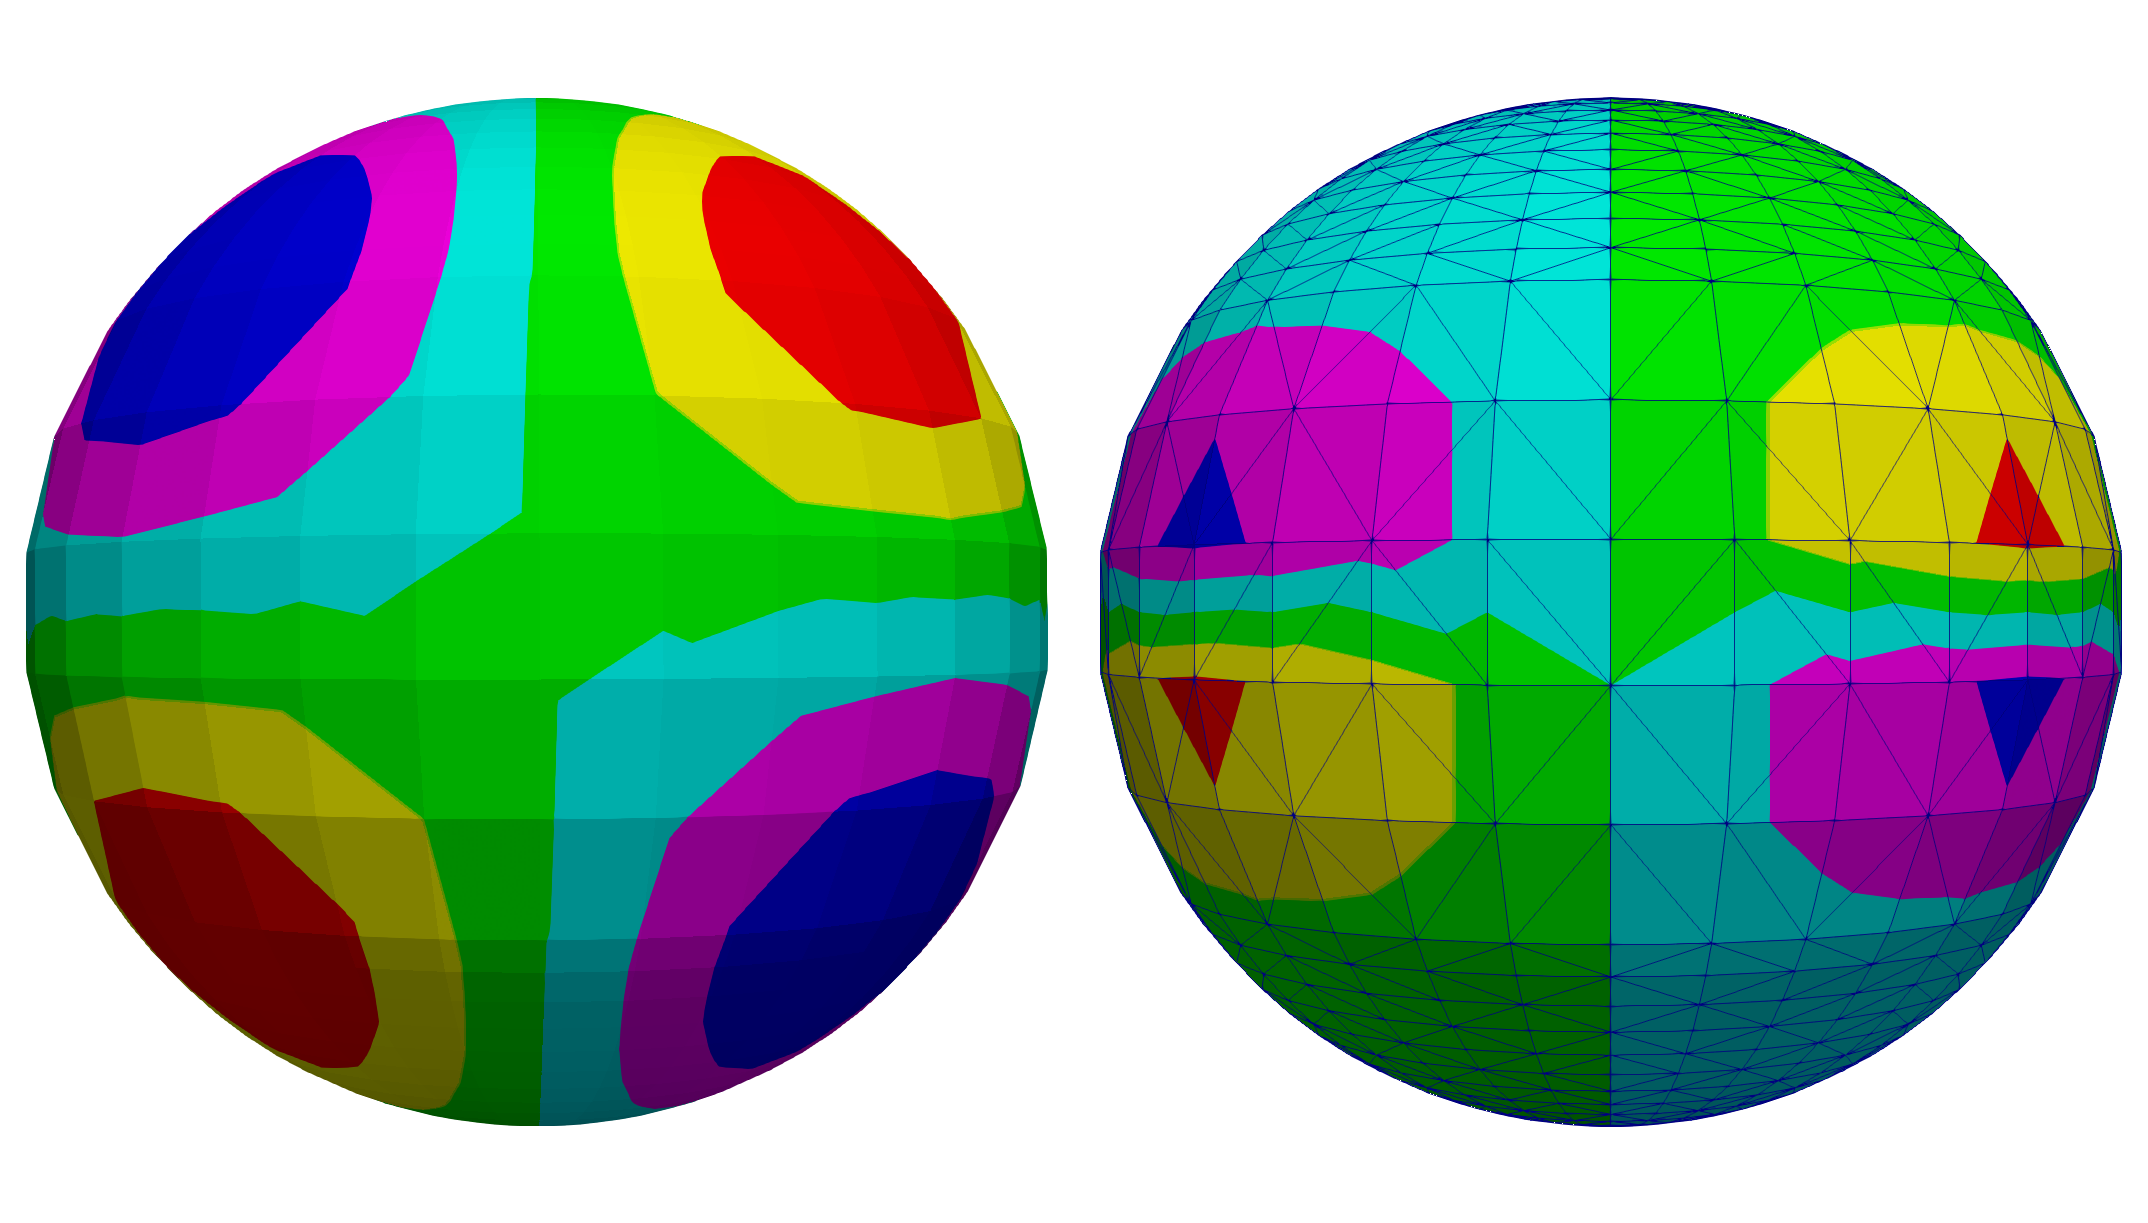
\includegraphics[width=0.7\textwidth]{../codes/04.imbalanced/img/confront_mixed.png}
	\end{center}
	\caption{\label{fig:equiangular distortion}On the left, the correct eigenmode. On the right: distortion of the eigenmode of the HKGL caused by an irregular sampling scheme of the sphere.}
\end{figure}
We can see that the eigenmodes end up being artificially compressed along the equator.
The goal of this chapter is to study a way of building a discrete approximation $\mathbf L$ of the Laplace-Beltrami operator more robust to non uniform sampling schemes than the HKGL $\mathbf L_n^t$ used so far.

This chapter is organized as follows: In Section \ref{sec:Chapter3: Heat Kernel Graph Laplacian on the Equiangular Sampling} we introduce the equiangular sampling and the results that we obtained with the HKGL. In Section \ref{sec:Chapter3: other discrete laplacians} we present a short overview of different ways of building a discrete approximation of the Laplace-Beltrami operator; in Section \ref{sec:Chapter3: Using the Finite Element Method to approximate the Laplace-Beltrami operator on a manifold} we deepen how to use the Finite Element Method (FEM) to construct a discrete approximation of $\triangle_{\mathbb S^2}$ and how it is actually capable of taking into account the non uniformity of the sampling scheme and correct it.
\subsection{Graph Laplacian on the Equiangular Sampling}
\label{sec:Chapter3: Heat Kernel Graph Laplacian on the Equiangular Sampling}

\subsubsection{The Equiangular Sampling}

Given the usual parametrization $x = x(\theta, \phi)$ of the sphere
\begin{align*}
	\mathbb{S}^{2}&=\left\{x=\left(x_{1}, x_{2}, x_{3}\right) \in \mathbb{R}^{3} :\|x\|_{\mathbb{R}^{3}}=\left(x_{1}^{2}+x_{2}^{2}+x_{3}^{2}\right)^{1 / 2}=1\right\}\\
	x_{1}&=\cos (\phi) \sin (\theta), \quad x_{2}=\sin (\phi) \sin (\theta), \quad x_{3}=\cos (\theta)
\end{align*}

Let $m\in\mathbb N$, the \textit{equiangular sampling} of bandwidth $b=2^m$ is given by 
$
x_{j k}^{(b)}=x\left(\theta_{j}^{(b)}, \phi_{k}^{(b)}\right)
$
where
\begin{align*}
	\theta_{j}^{(b)} &:=\pi \frac{j}{2 b}, \quad \phi_{k}^{(b)} :=2 \pi \frac{k}{2 b}\\
	j&=0, ..., 2b-1 \text{ and }k=0, ..., 2b-1 
\end{align*}

\begin{figure}[h]
	\centering
	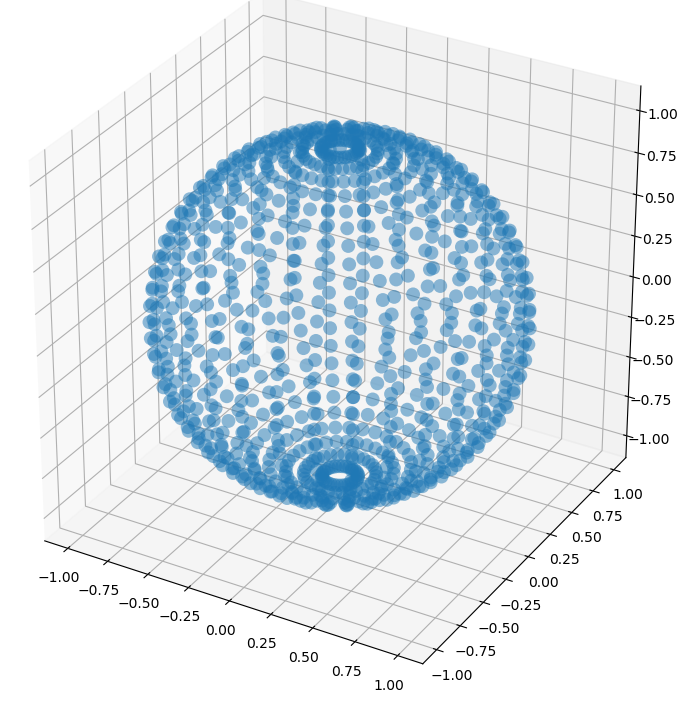
\includegraphics[width=0.5\textwidth]{figs/Chapter3/equiangular.png}
	\caption{\label{fig:equiangular sampling}Equiangular sampling with bandwidth $b=8$}
\end{figure}
One has thus $n=4b^2$ points on the sphere, where all the points $x_{0 k}^{(b)}$ correspond to the north pole for every $k=0, ..., 2b-1$. Notice also that the south pole is never sampled. In figure \ref{fig:equiangular sampling} it can also be appreciated how the area close to the poles is much more sampled that the equator. One reason for which this sampling scheme is very used in application is the existence of the following result from \cite{Driscoll:1994:CFT:184069.184073}, that states that any band limited function can be exactly recovered from its sampled values $f\left(x_{j k}^{(b)}\right)$:
\vspace{0.5cm}
\begin{theorem}\label{theo:equiangular sampling theorem}
	Let \(l_{0} \in \mathbb{N}\) and \(m_{0} \in \mathbb{Z},\left|m_{0}\right| \leq l_{0} .\) If \(f=\sum_{l=0}^{b-1} \sum_{m=-l}^{l} \widehat{f}(l, m) Y_{l}^{m}\)
	then
	
	$$
	\begin{aligned} \widehat{f}\left(l_{0}, m_{0}\right)=& \frac{1}{4 b^{2}} \sum_{j=0}^{2 b-1} \sum_{k=0}^{2 b-1} f\left(x_{j k}^{(b)}\right) \overline{Y_{l_{0}}^{m_{0}}\left(x_{j k}^{(b)}\right)} \sin \left(\theta_{j}^{(b)}\right) \times \\ & \times \frac{4}{\pi} \sum_{l=0}^{b-1} \frac{1}{2 l+1} \sin \left((2 l+1) \theta_{j}^{(b)}\right) \end{aligned}
	$$
\end{theorem}
\vspace{0.5cm}
Theorem \ref{theo:equiangular sampling theorem} is the equivalent on the sphere of the well known Shannon's sampling theorem, that states the minimum sampling frequency at which a band limited signal $f:\mathbb R \to \mathbb R$ can be perfectly reconstructed, and is a precious tool when doing signal processing on the sphere.

\subsubsection{Heat Kernel Graph Laplacian with non uniform sampling measures}
Thanks to Theorem \ref{theo:equiangular sampling theorem}, we can compute exactly the Fourier transform of the eigenmodes of the HKGL and see how much they are aligned with the eigenspaces of the true Laplace-Beltrami operator, following the same procedure described at the beginning of Chapter 2 when introducing the same kind of plots for the HEALPix sampling scheme. It can be appreciated how poorly aligned the eigenmodes of the HKGL are on the equiangular sampling (figure \ref{fig:equiangular sampling alignment}) compared to the ones obtained with the HEALPix sampling (\ref{fig:optimal graph})


\begin{table}[h!]
	\centering
	\begin{tabular}{ c|c } 
$b$ & $t$ \\ 
	\hline
4 & 0.5 \\ 
8 & 0.3 \\ 
16 & 0.1 \\ 
	\end{tabular}
	\caption{\label{table:equiangular kernel width}Kernel width $t$ used to construct the HKGL for each bandwidth $b$}
\end{table}

\begin{figure}[h!]
	\centering
	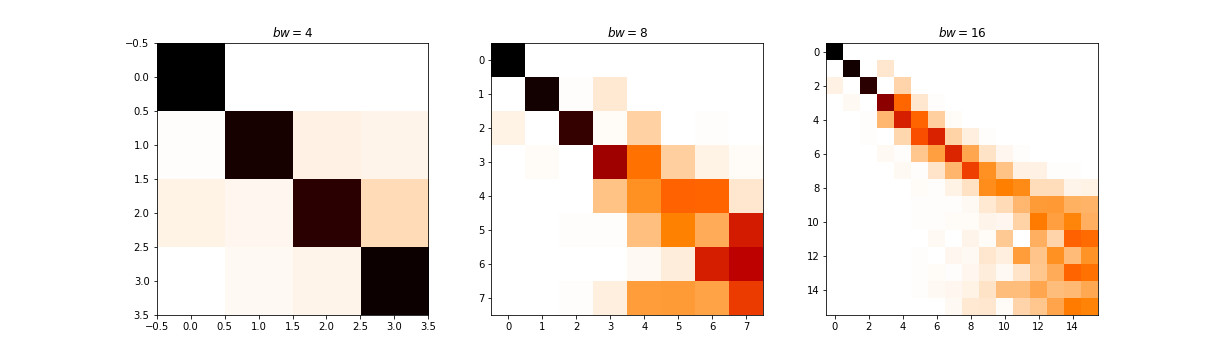
\includegraphics[width=0.9\textwidth]{../codes/02.HeatKernelGraphLaplacian/equiangular/equi_full.png}
	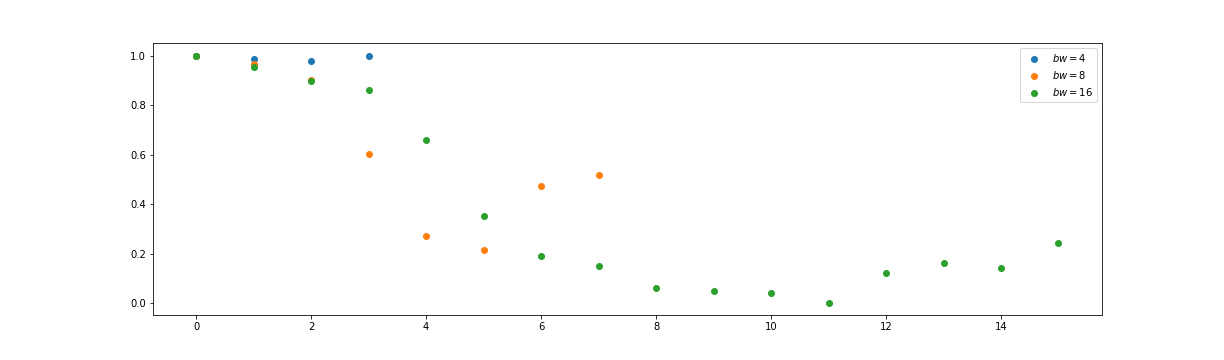
\includegraphics[width=0.9\textwidth]{../codes/02.HeatKernelGraphLaplacian/equiangular/equi_full_diagonal.png}
	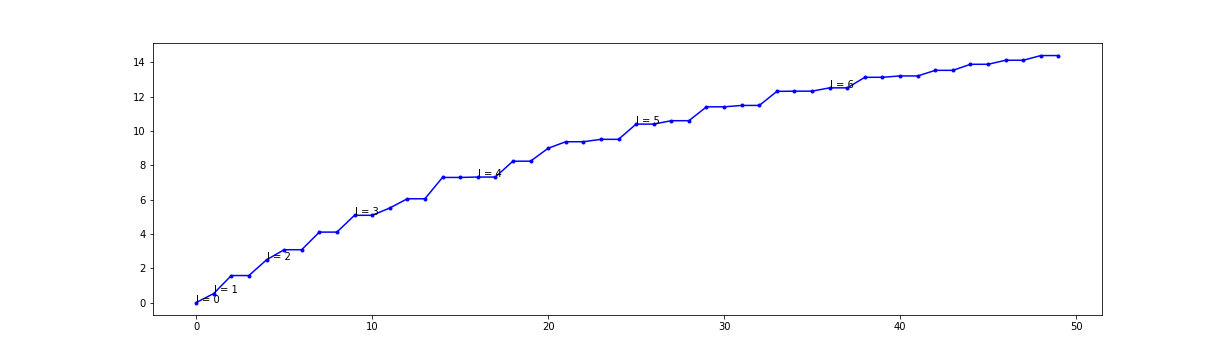
\includegraphics[width=0.9\textwidth]{../codes/02.HeatKernelGraphLaplacian/equiangular/equi_full_eigenvalues_16.png}
	\caption{\label{fig:equiangular sampling alignment}Alignment of eigenspaces of the full HKGL with respect to the true Laplace-Beltrami eigenspaces on the equiangular sampling. The kernel width for each bandwidth $bw$ are given by table \ref{table:equiangular kernel width}}
\end{figure}
The HKGL behaves badly in the case of the equiangular sampling, and does not seem to converge to $\triangle_{\mathbb S^2}$, thus making us think that the equiangular sampling does not respect the uniformity hypothesis of theorem \ref{theo:pointwise convergence in the healpix case}. The proof of Proposition 4 gives us a hint to understand the reasons behind this bad alignment of the eigenmodes. For convenience of notations define 
\begin{align*}
	\phi^{t}(x ; y):=e^{-\frac{||x-y||^2}{4t}}\left(f(y)-f(x)\right)
\end{align*}
 In order for theorem \ref{theo:pointwise convergence in the healpix case} to hold, Proposition 4 states that the HKGL operator $$L_n^tf(\mathbf y)=\sum_i \frac{1}{n} \phi^{t}(\mathbf x_i ; \mathbf y)$$ must well approximate the functional approximation of the Laplace-Beltrami operator $$L^tf(\mathbf y)=\int_\mathcal M\phi^{t}(\mathbf x ; \mathbf y)d\mu(\mathbf x)$$
 where $\mu(\mathbf x)$ is the \textit{uniform probability measure} on the sphere.
The way of building the HKGL works well with a random sampling scheme because in this case the HKGL is an \textit{unbiased estimator} of the operator $L^t$.

To conclude, we understood that in the case of a non uniform sampling measure the original way of Belkin et al. \cite{Belkin:2005:TTF:2138147.2138189} to construct the HKGL can not work any more, and we need an alternative way to construct a graph whose Laplacian can well approximate the Laplace Beltrami operator on $\mathbb S^2$. In the next section we present some different ways of building the discrete Laplacian matrix $\mathbf L$. Some of these do not even use the notion of graph but come from notions of Differential Geometry or Numerical Mathematics.

\subsubsection{A graph alternative to the HKGL for the equiangular sampling}

Frossard et al. \cite{Frossard2017GraphBasedCO} design a discrete Laplacian that is explicitly intended to work on the sphere with the equiangular sampling. They studied a way to build a graph to analyze images produced by omnidirectional cameras. In their work they assume that the image is sampled on the sphere on the equiangular sampling. They consider the set $\mathcal G$ of all the possible graphs where each node is connected only to four of its nearest neighbours (North, Sud, West, East) and propose a weighting scheme $w_{ij}$ specifically designed for the analysis of spherical signals. To design this weight scheme they minimize the difference in the response to the polynomial spectral filter $\mathcal F = \mathbf L$ evaluated on images of the same object seen at different latitudes. In other words, they solve the minimization problem

\begin{equation}\label{eq:minimization frossard}
	\min_{W\in\mathcal G} \left|\mathcal{F}\left(\mathbf{y}\left(v_{ e}\right)\right)-\mathcal{F}\left(\mathbf{y}\left(v_{ i}\right)\right)\right|
\end{equation}
\begin{figure}
	\begin{center}
		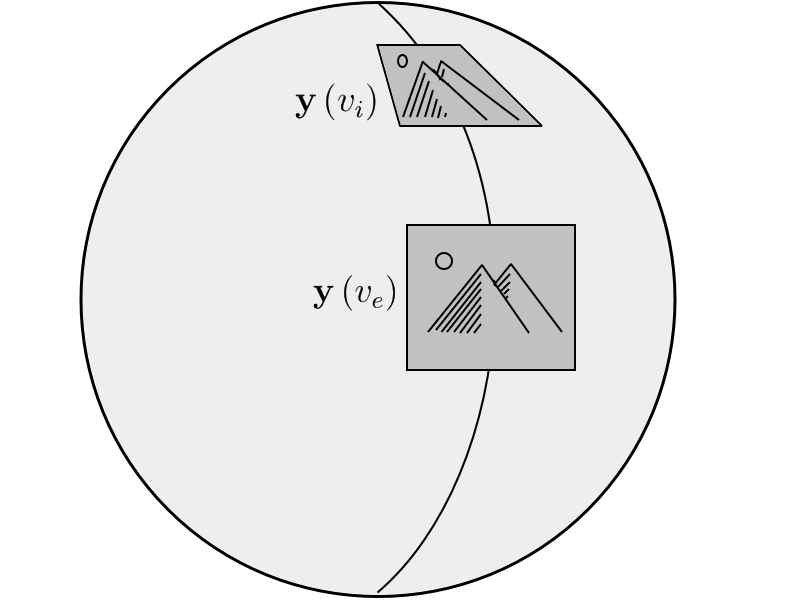
\includegraphics[width=0.5\textwidth]{figs/Chapter3/frossard2.png}
	\end{center}
	\caption{\label{fig:frossard2}Frossard et al. setting.}
\end{figure}
for the adjacency matrix $W$, where $\mathbf y(v_i)$ is the image of the object on the sphere centered on the vertex $v_i$, and $\mathcal F \mathbf y(v_e)$ is the response of the filter at the vertex $v_e$ that lies at the same longitude of the vertex $v_i$ but on the equator (figure \ref{fig:frossard2}). In their work they prove that the optimal weights solving the minimization problem (\ref{eq:minimization frossard}) are given by weights $w_{ij}$ inversely proportional to the Euclidean distance between vertices
\begin{equation}\label{eq:frossard weights}
	w_{ij} = \frac{1}{\norm{x_i-x_j}}
\end{equation}
This construction is interesting since it is adapted to the equiangular sampling (where the HKGL performed badly) and leads to a graph with only 4 neighbors per vertex, thus very sparse. Furthermore, to obtain the weights (\ref{eq:frossard weights}) every calculation was done in the \textit{spatial domain}, without any consideration about the spectral interpretation of the filter. In order to compare it to the HKGL we show the same Power Spectrum analysis in figure \ref{fig:Frossard/Khasanova graph}. It can be appreciated how this construction performs way better than the \textit{full} HKGL, having furthermore the big advantage of being naturally very sparse.
\begin{figure}[h!]
	\centering
	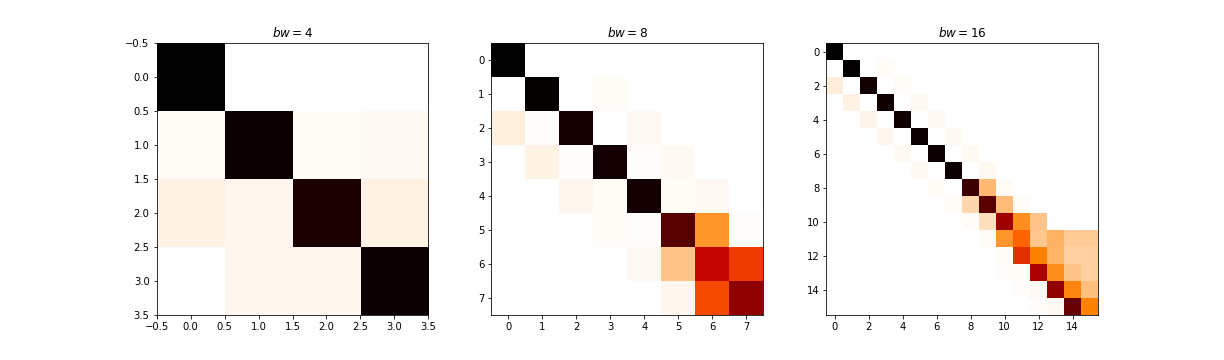
\includegraphics[width=0.9\textwidth]{../codes/02.HeatKernelGraphLaplacian/equiangular/equi_Khasanova_Frossard_full.png}
	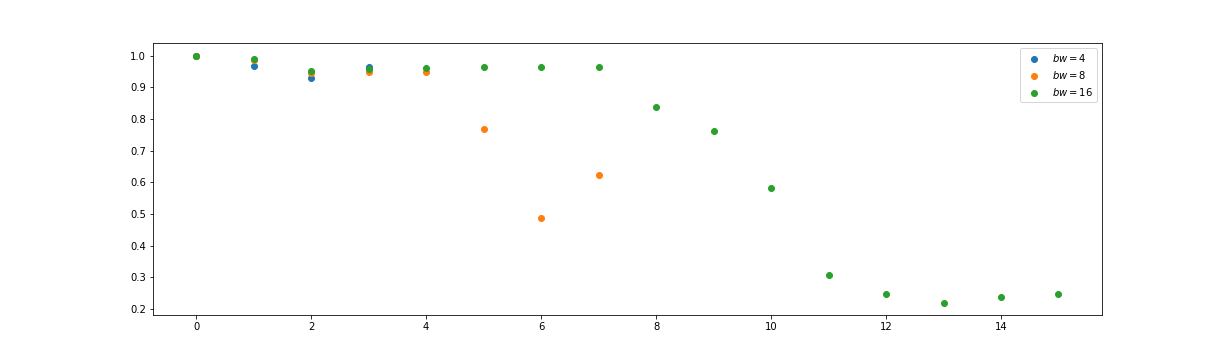
\includegraphics[width=0.9\textwidth]{../codes/02.HeatKernelGraphLaplacian/equiangular/equi_Khasanova_Frossard_full_diagonal.png}
	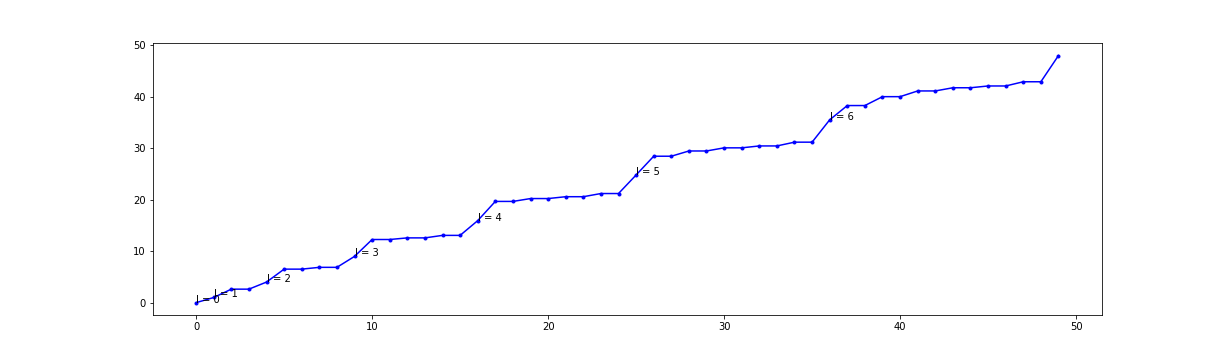
\includegraphics[width=0.9\textwidth]{../codes/02.HeatKernelGraphLaplacian/equiangular/equi_full_Khasanova_Frossard_eigenvalues_16.png}
	\caption{\label{fig:Frossard/Khasanova graph}Khasanova-Frossard graph}
\end{figure}

\subsection{The Finite Element Method approximation of the Laplace-Beltrami operator on a manifold}\label{sec:Chapter3: Using the Finite Element Method to approximate the Laplace-Beltrami operator on a manifold}
Given a differential operator $D$ and a Partial Differential Equation problem in the form
\begin{align}\label{eq:PDE}
\begin{split}
\text{Find } f(x):\Omega\in\mathbb R &\text{ such that, given }u(x):\Omega\to\mathbb R, g(x):\partial\Omega\to\mathbb R\\
Df(x)=u(x)\quad&x\in\Omega\\
f(x)=g(x)\quad &x\in\partial\Omega
\end{split}
\end{align}
the Finite Element Method (FEM) is a numerical algorithm that allows to calculate a discrete approximation of the solution $f$ through a functional discretization of the differential operator $D$. Even if in our setting we are not interested in PDE problems of the form \ref{eq:PDE}, we are interested in the FEM discretization of the differential operator $D=\Delta_{\mathbb S^2}$. we put the necessary definitions and mathematical concepts necessary to properly introduce the weak formulation of a differential problem, the Galerkin method and finally the Finite Element Method in Appendix.\\
\subsubsection{The FEM eigenvalue problem on the Sphere}\label{sec:Chapter3:FEM on the sphere}
Let's transform the strong form of the eigenvalue problem (\ref{eq:continous eigenvalue problem}) on the Sphere on its \textit{weak} formulation. Let's multiply equation (\ref{eq:continous eigenvalue problem}) by a sufficiently regular function $v$ and integrate on $\mathbb S^2$. Since the sphere is a closed manifold and has no border, integrating by parts yields
\begin{equation}\label{eq:weak eigenvalue problem}
\begin{split}
&\text{Find } f\in H^1(\mathbb S^2), \lambda\in\mathbb R\text{ such that }\\ 
&\int_{\mathbb S^2} \nabla f(\mathbf x)\cdot\nabla v(\mathbf x) d\mathbf x = \lambda \int_{\mathbb S^2} f(\mathbf x)\cdot v(\mathbf x)d\mathbf x\quad \forall v\in H^1(\mathbb S^2)
\end{split}
\end{equation}
with no boundary conditions, where $H^1\subset L^2(\mathbb S^2)$ is the Sobolev space of all the functions with derivative $\nabla f\in L^2(\mathbb S^2)$. The Finite Element Method first approximates the domain $\Omega$ with a triangulation $\mathcal T_h$, and then \textit{projects} the weak problem (\ref{eq:weak eigenvalue problem}) into a finite dimensional subspace $V_h\subset H^1(\mathcal T_h)$ made by all the piecewise linear polynomials on the triangulation $\mathcal T_h$. Define 
$$X_h^{1}=\{v_h: v_h\in C(\Omega): \left.v_h\right|_{\tau}\in\mathbb P^1\  \forall \tau\in \mathcal T_h\}$$
to be the space of all the continuous, piecewise linear functions on $\Omega$. A reasonable choice for $V_h$ is the space $X_h^{1,0}\subset H_0^1(\Omega)$ of the functions of $X_h^1$ that vanish on $\partial \mathcal T_h$
$$
X_h^{1,0}=\{v_h: v_h\in C(\Omega): \left.v_h\right|_{\tau}\in\mathbb P^1\  \forall \tau\in \mathcal T_h, \left.v_h\right|_{\partial\Omega}=0\}
$$ 
Since for the functions in $X_h^1$ the number of degrees of freedom is the same of the number of vertices of the mesh $n$, we need  $n$ basis functions $\phi_i, i=0,...,n-1$ to fully describe $X_h^{1}$. The most natural choice for $\phi_i$ is the following: $\phi_i$ is defined as the continuous piecewise linear function such that 
$$
\phi_i(x_j) = \delta_{ij}\quad i=0,...,n-1
$$
The support of $\phi_i$, i.e. the subset of $\mathcal T_h$ where $\phi_i$ is not zero is made by all the triangles sharing the $i$th vertex. An example is shown in figure \ref{fig:basis function}. To obtain a basis for the smaller space $X_h^{1,0}\subset X_h^{1}$ we just not take into account those $\phi_i$ that assume positive values on the vertices belonging to the border $\partial\Omega$. 

\vspace{0.5cm}
\begin{remark}
	For a function $v_h \in X^1_h,\ v_h = v_0 \phi_0 +...  v_n \phi_n$ the coefficient $v_i$ is equal to the function $v_h$ evaluated in the $i$th vertex 
	\begin{equation}\label{eq:dof and values}
	v_i = v_h(\mathbf x_i)
	\end{equation}
\end{remark}\vspace{0.5cm}
\begin{figure}[h]
	\begin{center}
		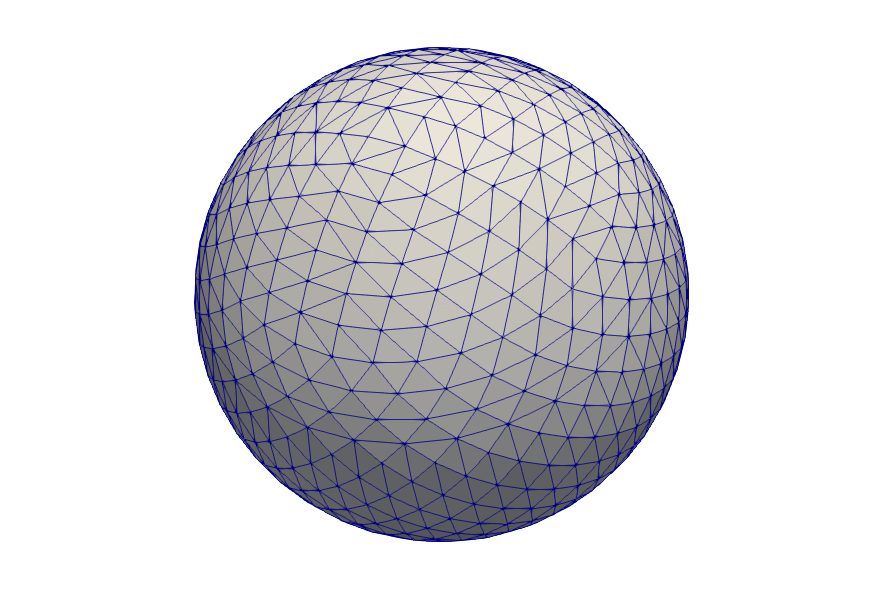
\includegraphics[width=0.6\textwidth]{figs/Chapter3/sphere_mesh.png}
	\end{center}
	\caption{\label{fig:sphere mesh}A triangulation $\mathcal T_h$ of the sphere made with the vertices of the HEALPix sampling with $N_{side}=8$}
\end{figure}
\begin{figure}
	\begin{center}
		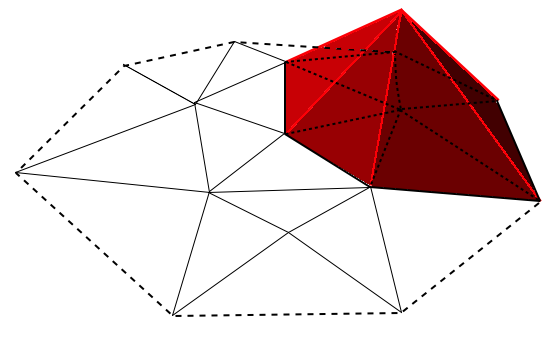
\includegraphics[width=0.4\textwidth]{figs/Chapter3/basisfunction.png}
	\end{center}
	\caption{\label{fig:basis function}Basis function of the space $X^{1}_h$}
\end{figure}

By writing $n$ times the equation (\ref{eq:weak eigenvalue problem}), setting each time the test function $v_h$ equal to the $i$th basis function $\phi_i$ of the space $X_h^1$, we obtain the generalized algebraic eigenvalue problem
\begin{align}\label{eq:algebraic generalized eigenvalue problem}
	&\text{Find }(f,\lambda)\text{ such that }A\mathbf f = \lambda B \mathbf f\\
	&\begin{cases}
	(A)_{ij} &= \int_{\mathbb S^2}\nabla \phi_i(\mathbf{x})\cdot \nabla \phi_j(\mathbf{x})d\mathbf{x}\\
	(B)_{ij} &= \int_{\mathbb S^2} \phi_i(\mathbf{x}) \phi_j(\mathbf{x})d\mathbf{x}\\
	(\mathbf f)_i &= f_i:\quad f(\mathbf x) = f_0\phi_0(\mathbf x)+ ... + f_{n-1}\phi_{n-1}(\mathbf x) 
	\end{cases}
\end{align}
Observe that being the Laplace-Beltrami operator self-adjoint, we have that $A=A^T, B=B^T$. Being $B$ non singular, the system (\ref{eq:algebraic generalized eigenvalue problem}) is equivalent to the eigenvalue problem
\begin{equation}\label{eq:algebraic  eigenvalue problem}
B^{-1}A\mathbf f = \lambda \mathbf f
\end{equation}



Taken any triangulation of the sphere $\mathcal T_h$, since $\mathbb S^2$ does not have boundaries and thus there are no boundary conditions to impose, this time the correct space $V_h$ to chose is $X^1_h$. The number of degrees of freedom of the space - and thus the number of basis functions - is equal to the number of vertices of the mesh and thanks to equation (\ref{eq:dof and values}) the solution $\mathbf f$ that is the vector of the coefficients of the function $f_h$ in the basis $\phi_i$ corresponds exactly to the values of the function $f_h$ in the vertices. For these reasons, the matrix $\mathbf L$ that we are looking for to perform our graph-like convolution is exactly
$$
\mathbf L = B^{-1}A
$$
However, having chosen a basis $\{\phi_i\}_i$ not orthonormal, $B$ is different to the identity matrix and its inverse is full, making $\mathbf L$ not efficient to perform graph-like convolutions. However this is a well known problem in the FEM literature; a common workaround is the so called \textit{lumping} of the mass matrix, that consist in replacing the matrix $B$ with the \textit{lumped} diagonal matrix $D$ obtained by placing in each diagonal entry $(D)_{ii}$ the sum of the elements of the i-th row of the mass matrix $B$:

\begin{equation}\label{eq:lumping}
D = \text{diag}\{d_i\},\quad d_i = \sum_j (B)_{ij}
\end{equation}

This approximation is well studied in the literature and it is proved to work well in many practical cases. The inverse of the lumped mass matrix is diagonal as well $D^{-1} = \text{diag}\{\frac{1}{d_i}\}$ and thus the matrix $D^{-1}A$ in the lumped eigenvalue problem 
\begin{equation}\label{eq:lumped eigenvalue problem}
	D^{-1}A\mathbf f = \lambda \mathbf f
\end{equation}
has the same sparsity pattern of the stiffness matrix $A$, and thus leads to an acceptable computational cost of the filtering operation. However, $D^{-1}A$ is not symmetric; we then tried to use the symmetric matrix $\mathbf L = D^{-1/2}AD^{-1/2}$, thus solving the problem 
\begin{equation}\label{eq:symmetric lumped eigenvalue problem}
D^{-1/2}AD^{-1/2}\mathbf f = \lambda \mathbf f
\end{equation}
obtaining very promising results.
We implemented the eigenvalue problem \ref{eq:weak eigenvalue problem} in $X_h^1$. We show in figures \ref{fig:FEMHealpix}, \ref{fig:FEMequiangular} the usual analysis of the alignment of the eigenmodes for both HEALPix sampling and the equiangular sampling. Being the sphere convex, in both cases the mesh $\mathcal T_h$ has been obtained by calculating the triangulation of the convex hull of the vertices through the Qhull algorithm \cite{Barber96thequickhull}.

\begin{minipage}[t!]{.49\textwidth}
	\raggedleft
	\center
	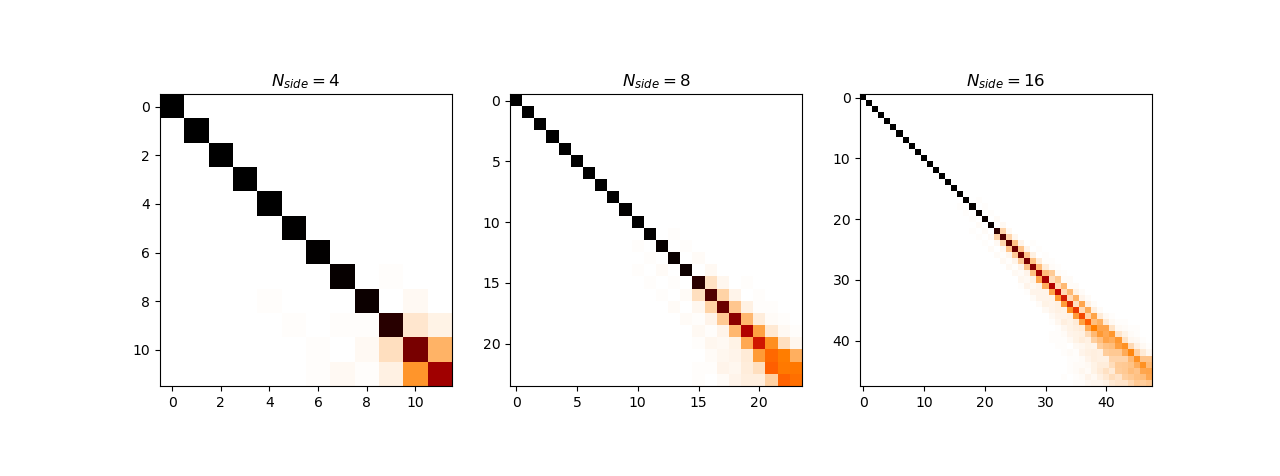
\includegraphics[width=\linewidth]{../codes/03.FEM_laplacian/HEALPix/img/linearFEM.png}\\
	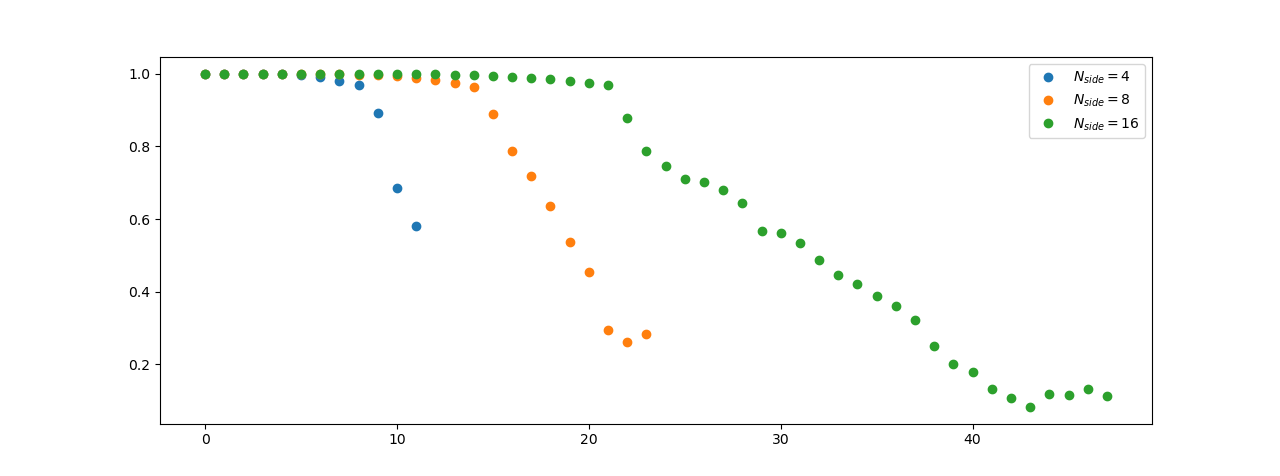
\includegraphics[width=\linewidth]{../codes/03.FEM_laplacian/HEALPix/img/linearFEM_diagonal.png}	\\
	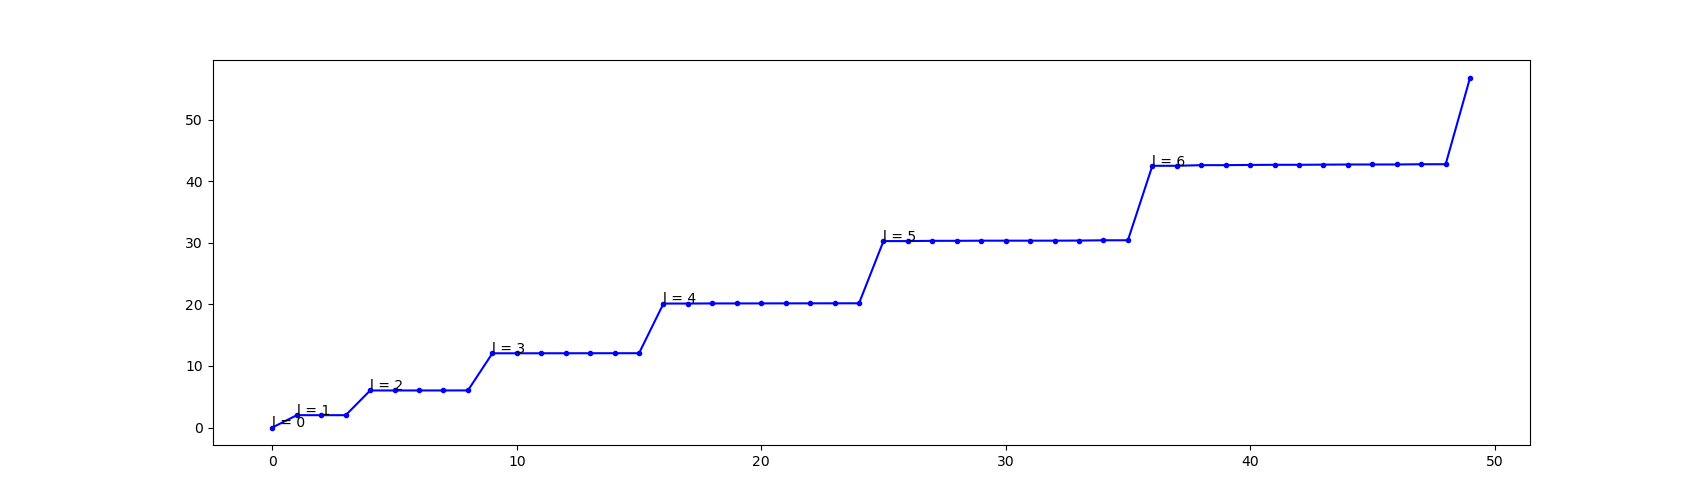
\includegraphics[width=\linewidth]{../codes/03.FEM_laplacian/HEALPix/img/FEM_eigenvalues_16.png}	\\
	\captionof{figure}{	\label{fig:FEMHealpix}Alignment of eigenspaces using the linear FEM approximation to solve the eigenvalue problem \ref{eq:algebraic  eigenvalue problem} on HEALPix}
\end{minipage}
\hfill
%
\begin{minipage}[t!]{.49\textwidth}
	\raggedright
	\center
	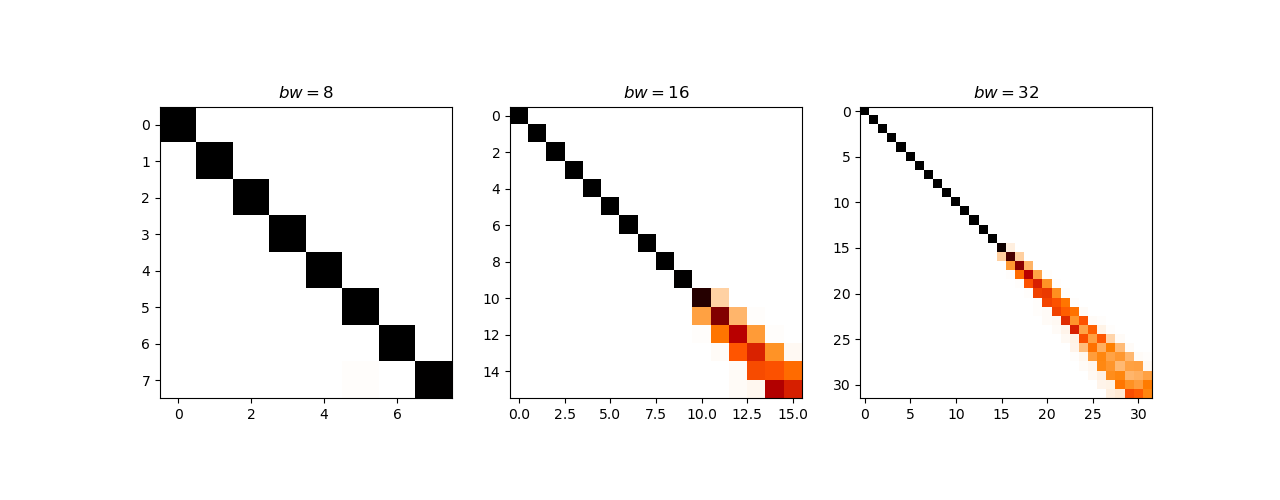
\includegraphics[width=\linewidth]{../codes/03.FEM_laplacian/equiangular/normal/img/linearFEM.png}
	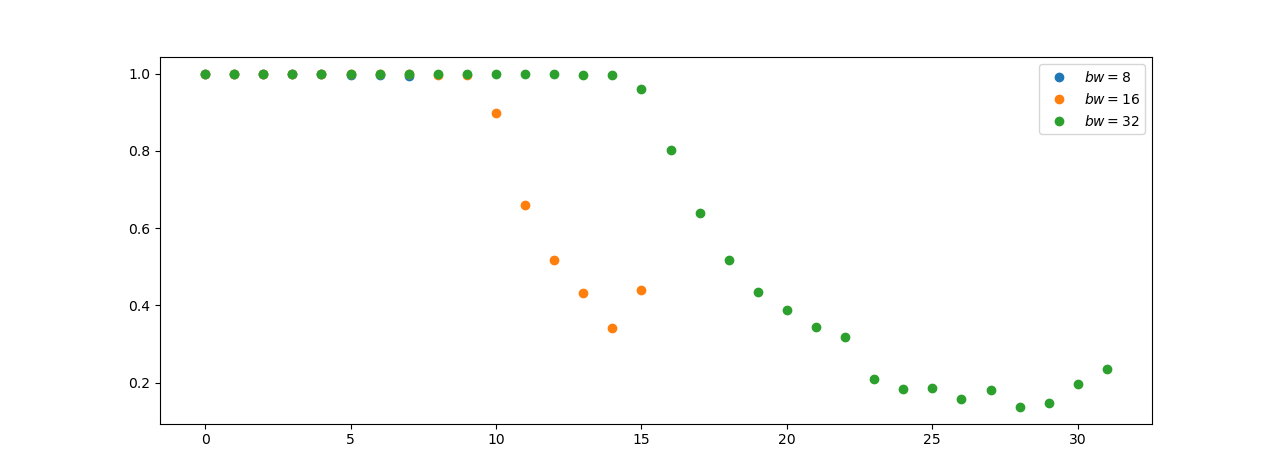
\includegraphics[width=\linewidth]{../codes/03.FEM_laplacian/equiangular/normal/img/linearFEM_diagonal.png}	
	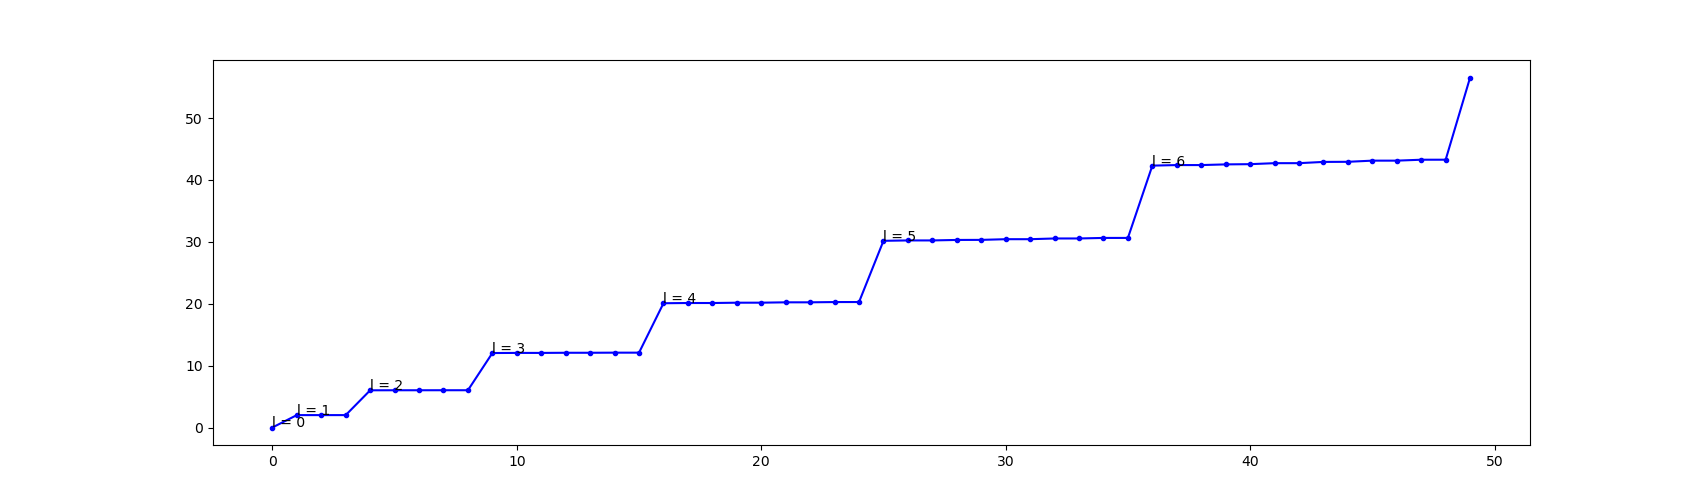
\includegraphics[width=\linewidth]{../codes/03.FEM_laplacian/equiangular/normal/img/FEM_eigenvalues_16.png}	
	\captionof{figure}{\label{fig:FEMequiangular}Alignment of eigenspaces using the linear FEM approximation to solve the eigenvalue problem \ref{eq:algebraic  eigenvalue problem} on the equiangular sampling}
\end{minipage}
\begin{minipage}[t!]{.49\textwidth}
	\raggedleft
	\center
	\centering
	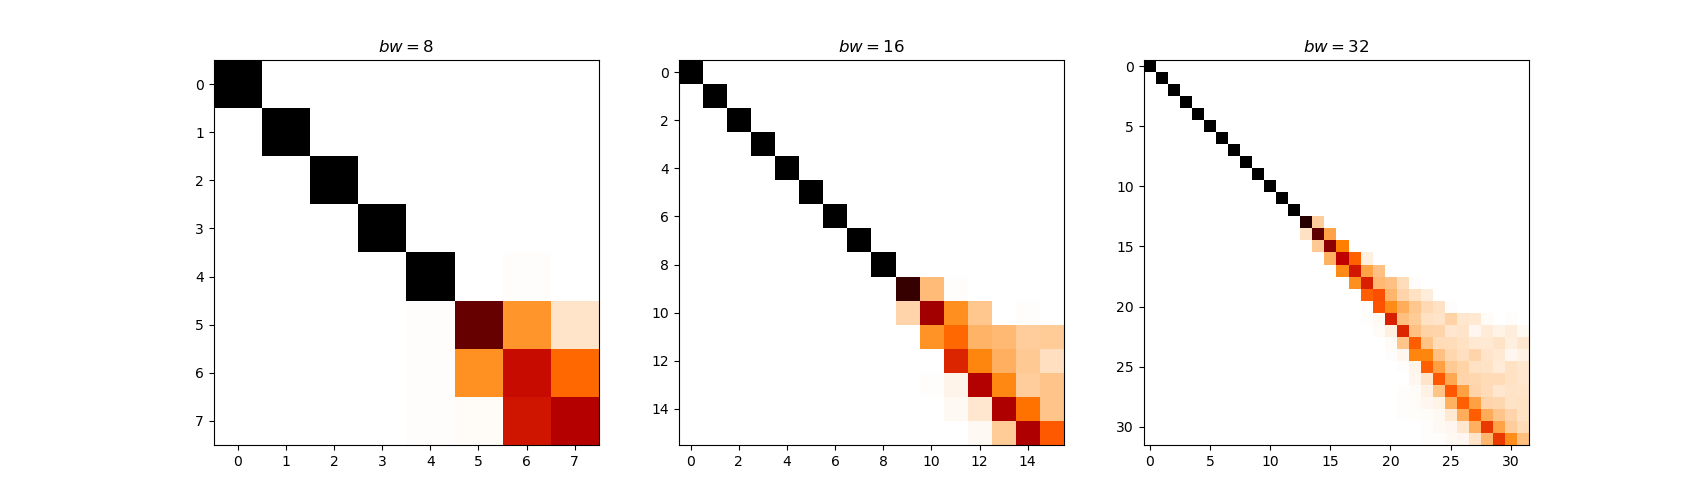
\includegraphics[width=\textwidth]{../codes/03.FEM_laplacian/equiangular/mass_lumping/BL/img/linearFEM.png}
	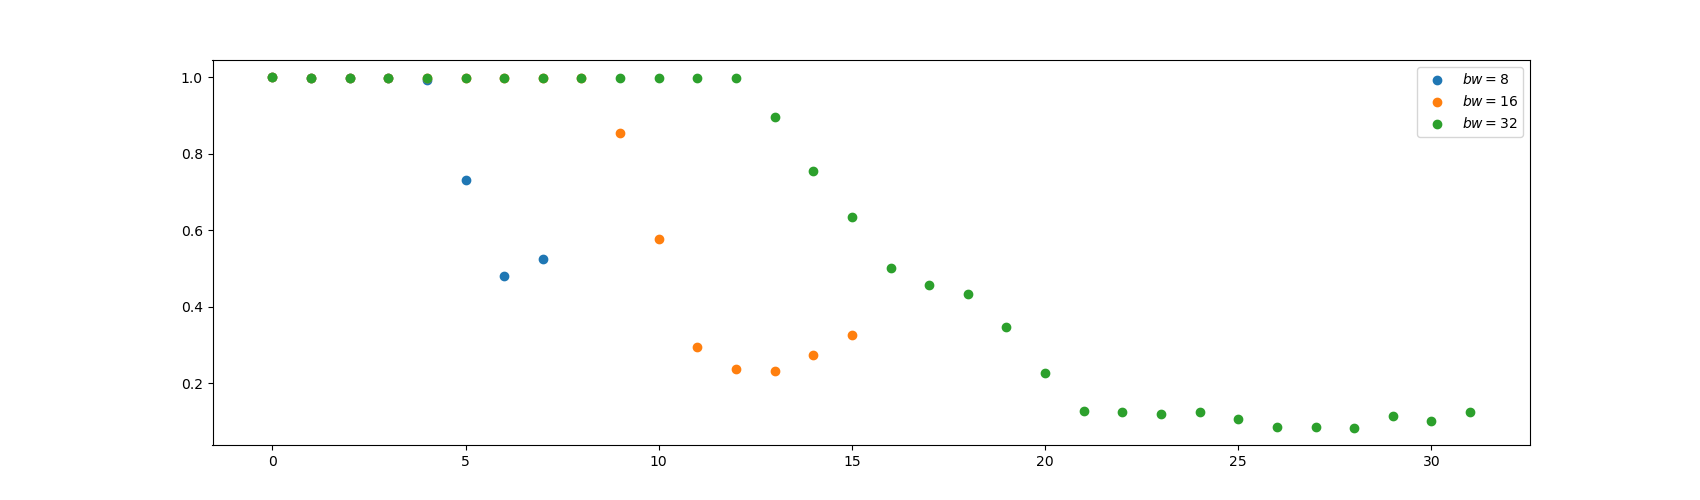
\includegraphics[width=\textwidth]{../codes/03.FEM_laplacian/equiangular/mass_lumping/BL/img/linearFEM_diagonal.png}	
	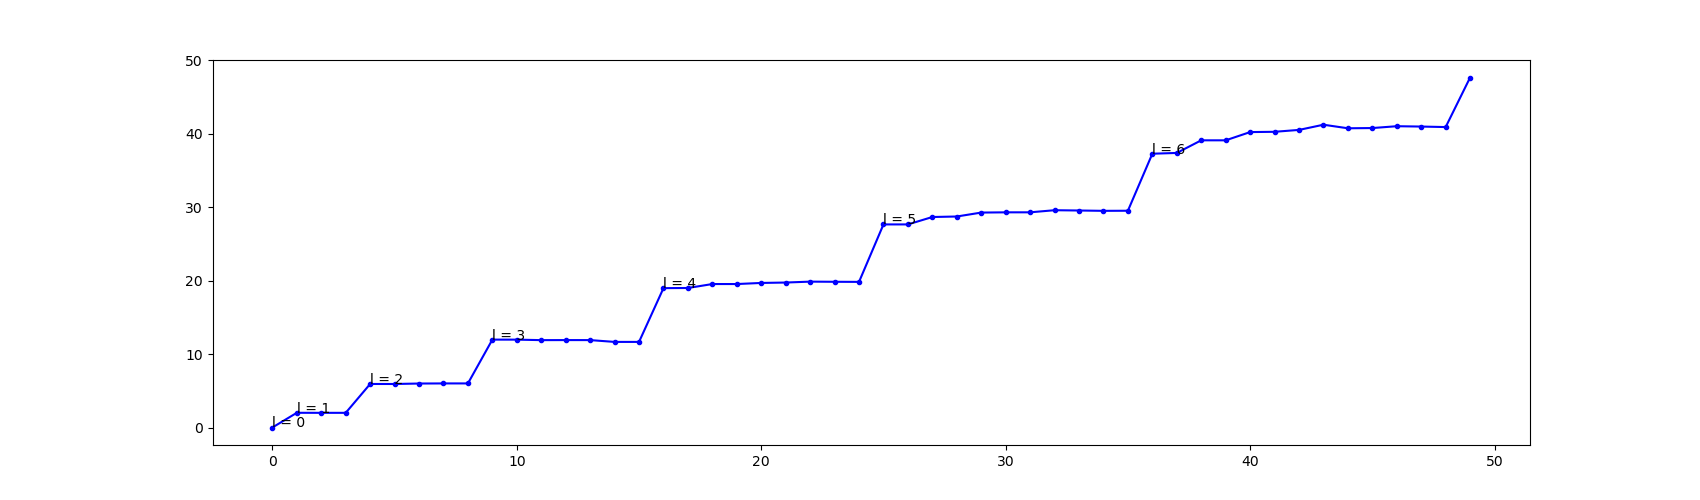
\includegraphics[width=\textwidth]{../codes/03.FEM_laplacian/equiangular/mass_lumping/BL/img/FEM_eigenvalues_32.png}	
	\captionof{figure}{\label{fig:FEMequiangularLumped}Alignment of eigenspaces using the linear FEM approximation to solve the \textit{lumped} eigenvalue problem \ref{eq:lumped eigenvalue problem} on the equiangular sampling}
\end{minipage}
\hfill
%
\begin{minipage}[t!]{.49\textwidth}
	\raggedright
	\center
	\centering
	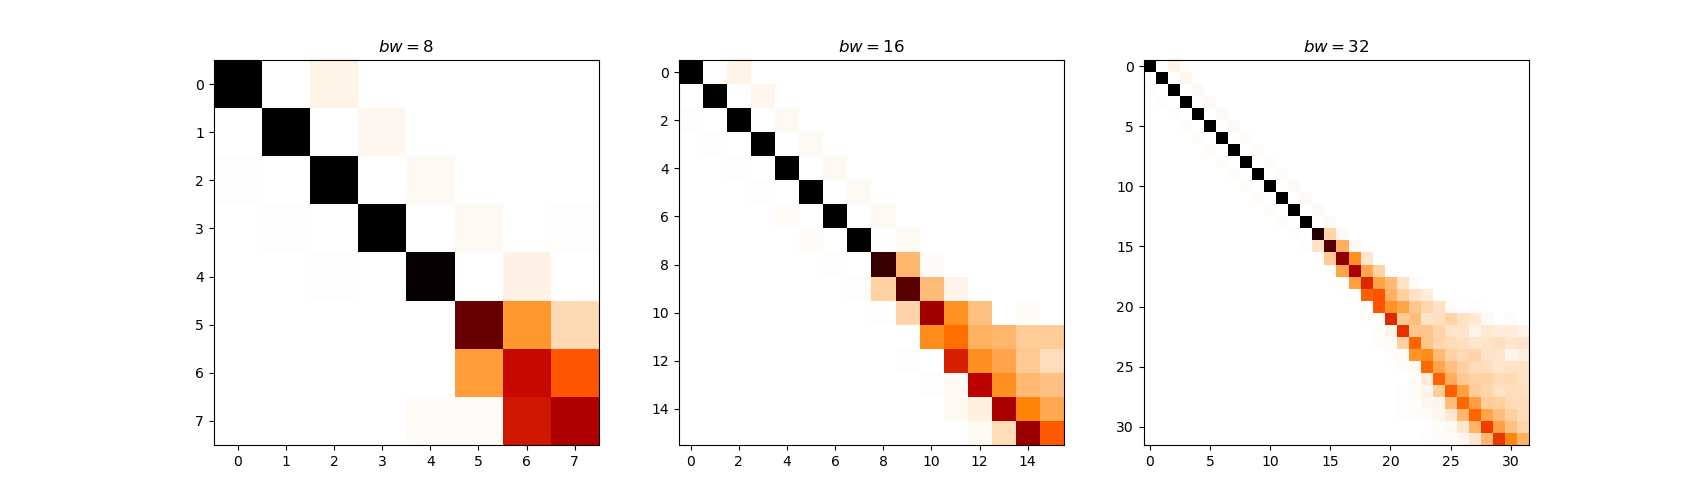
\includegraphics[width=\textwidth]{../codes/03.FEM_laplacian/equiangular/mass_lumping/BLB/img/linearFEM.png}
	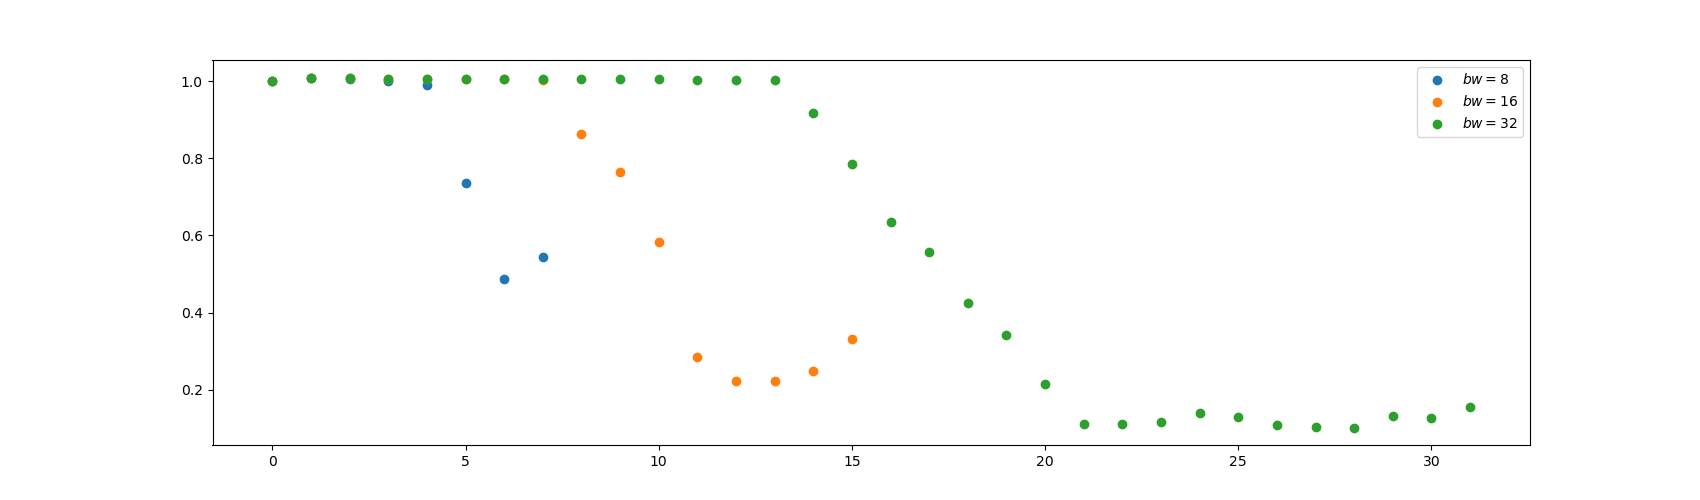
\includegraphics[width=\textwidth]{../codes/03.FEM_laplacian/equiangular/mass_lumping/BLB/img/linearFEM_diagonal.png}	
	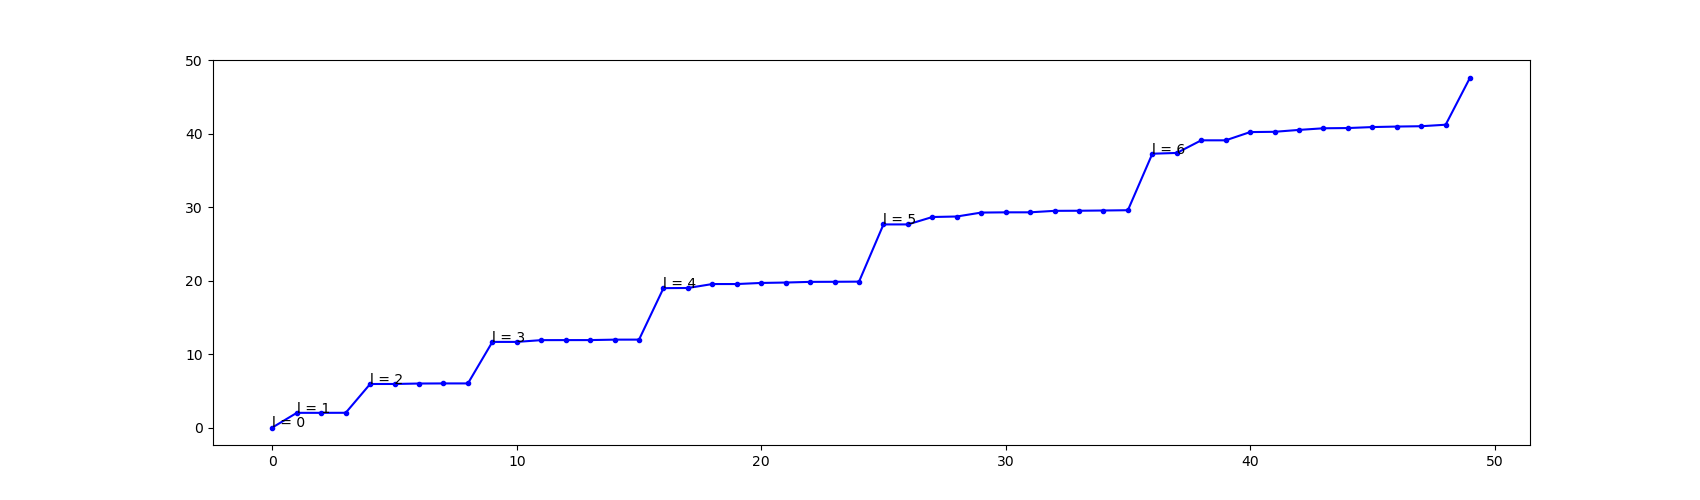
\includegraphics[width=\textwidth]{../codes/03.FEM_laplacian/equiangular/mass_lumping/BLB/img/FEM_eigenvalues_32.png}	
	\captionof{figure}{\label{fig:symmetricFEMequiangularLumped}Alignment of eigenspaces using the linear FEM approximation to solve the \textit{symmetric lumped} eigenvalue problem \ref{eq:symmetric lumped eigenvalue problem} on the equiangular sampling}
\end{minipage}

We see that on HEALPix the \textit{full} HKGL shows better aligned eigenmodes than the \textit{full} FEM Laplacian $B^{-1}L$. On the equiangular sampling the FEM shows its capability of catching the geometry of the problem independently of the sampling scheme (figure \ref{fig:FEMequiangular}). Furthermore it can be seen how on the equiangular sampling the solutions of the lumped Laplacian $D^{-1}L$ - figure \ref{fig:FEMequiangularLumped} - and of the symmetric lumped Laplacian $D^{-1/2}LD^{-1/2}$ - figure \ref{fig:symmetricFEMequiangularLumped} - look very close to the correct solution of the problem \ref{eq:algebraic  eigenvalue problem}, thus making the FEM approach very promising.



\subsubsection{Diffusion with the exponential matrix}

To show that it is possible to filter a signal with the matrix $\mathbf L = D^{-1/2}AD^{-1/2}$ in the graph-like way and to confront it to the full HKGL we filter a unit mass signal $\mathbf{f}=(0,0,...0,1,0,...,0)^T$ with the \textit{diffusion} filter $\exp{(-\tau \mathbf L)}$. To enhance the deformation caused by the HKGL it was chosen a very irregular sampling scheme, shown in figure \ref{fig:FEM lumped symmetric diffusion on irregular sampling}. It can be seen how the full HKGL compresses the signal around the equator where the sampling scheme is more sparse; on the other hand the FEM filtering manages to keep the diffusion homogeneous no matter the asymmetry in the sampling scheme. 
\begin{figure}[h]
	\centering
	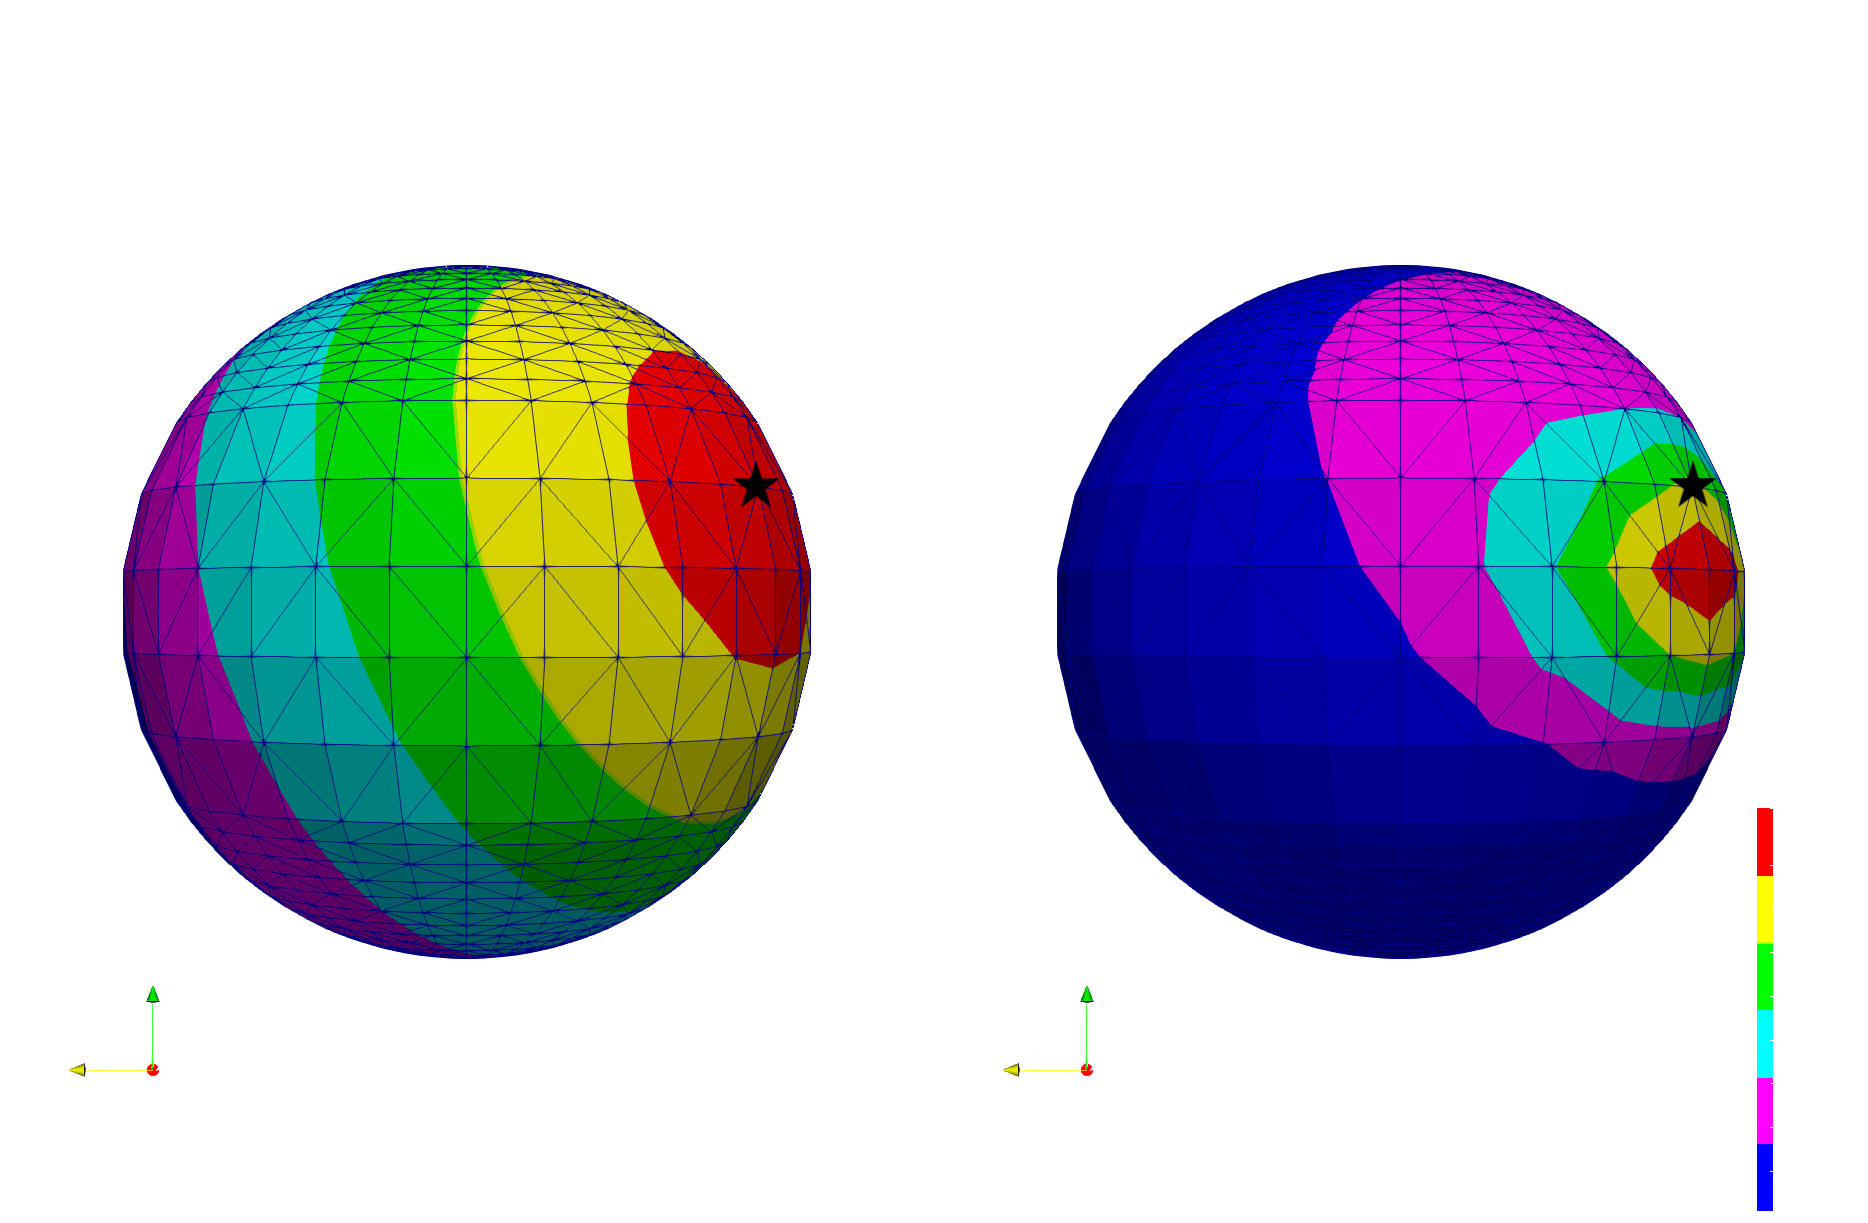
\includegraphics[width=0.8\textwidth]{figs/Chapter3/diffusion.png}
	\caption{\label{fig:FEM lumped symmetric diffusion on irregular sampling}Symmetric lumped linear FEM diffusion and HKGL diffusion on an irregular sampling scheme of the sphere. The position of the filtered source signal is indicated with a black star.}
\end{figure}






